\documentclass{article}

\usepackage{fancyhdr}
\usepackage{wrapfig}
\usepackage{extramarks}
\usepackage{multicol}
\usepackage{amsmath}
\usepackage{amsthm}
\usepackage{amsfonts}
\usepackage{tikz}
\usepackage{forest,adjustbox}
\usepackage[plain]{algorithm}
\usepackage{algpseudocode}
\usepackage{enumerate}
\usepackage[shortlabels]{enumitem}                     
          \setlist[enumerate, 1]{1\textsuperscript{o}}



\usepackage{listings}
\usepackage{xcolor}
%\lstset { %
%  language=C++,
%  backgroundcolor=\color{black!5}, % set backgroundcolor
%  basicstyle=\footnotesize,% basic font setting
%}

%\usetikzlibrary{automata,positioning}
\usetikzlibrary{positioning,shapes,shadows,arrows,automata} %
% Basic Document Settings
%

\topmargin=-0.45in
\evensidemargin=0in
\oddsidemargin=0in
\textwidth=6.5in
\textheight=9.0in
\headsep=0.25in

\linespread{1.1}

\pagestyle{fancy}
\lhead{\hmwkClass}
\chead{ (\hmwkClassInstructor\ \hmwkClassTime) }
\rhead{\shortName \hspace{0.4cm} \hmwkTitle}
\lfoot{\lastxmark}
\cfoot{\thepage}

\renewcommand\headrulewidth{0.4pt}
\renewcommand\footrulewidth{0.4pt}

\newcommand\curl[1]{\{#1\}}

\setlength\parindent{0pt}

%
% Create Problem Sections
%

\newcommand{\enterProblemHeader}[1]{
  \nobreak\extramarks{}{Problem \arabic{#1} continued on next page\ldots}\nobreak{}
  \nobreak\extramarks{Problem \arabic{#1} (continued)}{Problem \arabic{#1} continued on next page\ldots}\nobreak{}
}

\newcommand{\exitProblemHeader}[1]{
  \nobreak\extramarks{Problem \arabic{#1} (continued)}{Problem \arabic{#1} continued on next page\ldots}\nobreak{}
  \stepcounter{#1}
  \nobreak\extramarks{Problem \arabic{#1}}{}\nobreak{}
}

\setcounter{secnumdepth}{0}
\newcounter{partCounter}
\newcounter{homeworkProblemCounter}
\setcounter{homeworkProblemCounter}{1}
\nobreak\extramarks{Problem \arabic{homeworkProblemCounter}}{}\nobreak{}

%
% Homework Problem Environment
%
% This environment takes an optional argument. When given, it will adjust the
% problem counter. This is useful for when the problems given for your
% assignment aren't sequential. See the last 3 problems of this template for an
% example.
%
\newenvironment{homeworkProblem}[1][-1]{
  \ifnum#1>0
    \setcounter{homeworkProblemCounter}{#1}
  \fi
  \section{Problem \arabic{homeworkProblemCounter}}
  \setcounter{partCounter}{1}
  \enterProblemHeader{homeworkProblemCounter}
}{
  \exitProblemHeader{homeworkProblemCounter}
}

%
% Homework Details
%  - Title
%  - Due date
%  - Class
%  - Section/Time
%  - Instructor
%  - Author
%

\newcommand{\hmwkTitle}{Homework\ \#4}
\newcommand{\hmwkDueDate}{February 22 2016}
\newcommand{\hmwkClass}{CS581 Theory of Computation}
\newcommand{\hmwkClassTime}{Winter 2016}
\newcommand{\hmwkClassInstructor}{Harry H. Porter}
\newcommand{\hmwkAuthorName}{Konstantin Macarenco}
\newcommand{\shortName}{Konstantin M.}

%
% Title Page
%

\title{
  \vspace{2in}
  \textmd{\textbf{\hmwkClass:\ \hmwkTitle}}\\
  \normalsize\vspace{0.1in}\small{Due\ on\ \hmwkDueDate\ at 2:00pm}\\
  \vspace{0.1in}\large{\textit{\hmwkClassInstructor\ \hmwkClassTime}}
  \vspace{3in}
}

\author{\textbf{\hmwkAuthorName}}
\date{}

\renewcommand{\part}[1]{\textbf{\large Part \Alph{partCounter}}\stepcounter{partCounter}\\}
\newcommand{\answ}[1]{\hspace{1cm}\textbf{Answ:} #1}
\newcommand{\problem}[1]{\large{\textbf{Problem #1}}\\}

%
% Various Helper Commands
%

% Useful for algorithms
\newcommand{\alg}[1]{\textsc{\bfseries \footnotesize #1}}

% For derivatives
\newcommand{\deriv}[1]{\frac{\mathrm{d}}{\mathrm{d}x} (#1)}

% For partial derivatives
\newcommand{\pderiv}[2]{\frac{\partial}{\partial #1} (#2)}

% Integral dx
\newcommand{\dx}{\mathrm{d}x}

% Alias for the Solution section header
\newcommand{\solution}{\textbf{\large Solution}}

% Probability commands: Expectation, Variance, Covariance, Bias
\newcommand{\E}{\mathrm{E}}
\newcommand{\Var}{\mathrm{Var}}
\newcommand{\Cov}{\mathrm{Cov}}
\newcommand{\Bias}{\mathrm{Bias}}

\newcommand\Vtextvisiblespace[1][.3em]{%
  \mbox{\kern.06em\vrule height.3ex}%
  \vbox{\hrule width#1}%
  \hbox{\vrule height.3ex}}

\begin{document}

\maketitle

\pagebreak

\problem{4.1} \\
Answer all parts for the following DFA M and give reasons for your answers.

{\centering
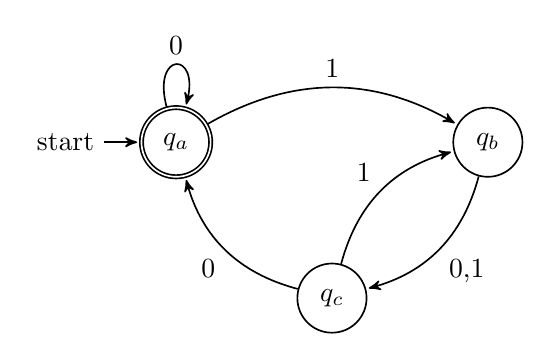
\begin{tikzpicture}[->,>=stealth',shorten >=1pt,auto,node distance=2.8cm,
                    semithick, transform shape, scale = 1]
  \tikzstyle{every state}=[fill=none,draw=black,text=black]

  \node[initial,state, accepting]     (A)                    {$q_a$};
  \node[state]             (C) [below right of=A ]       {$q_c$};
  \node[state]             (B) [above right of=C]       {$q_b$};

  \path (A) edge [bend left]  node [align=center] {1}   (B)
            edge [loop above] node [align=center] {0}   (A)
        (B) edge [bend left]  node [align=center] {0,1} (C)
        (C) edge [bend left]  node [align=center] {1}   (B)
            edge [bend left]  node [align=center] {0}   (A);
\end{tikzpicture}

}

\begin{enumerate}[1., leftmargin = 1.5cm]
\itemsep0em
\item Is $\langle M,0100 \rangle \in A_{DFA}$?\\
    Yes. The DFA M accepts 0100.
\item Is $\langle M,011 \rangle \in A_{DFA}$?
    No. The DFA M doesn't accept 011.
\item Is $\langle M \rangle \in A_{DFA}$?
    No. This input has only a single component and thus is not of the correct form.
\item Is $\langle M,0100 \rangle \in A_{REX}$?
    No. The first component is not a regular expression and so the input is not of the correct form.
\item Is $\langle M \rangle \in E_{DFA}$?
    No. M's language isn't empty.
\item Is $\langle M,M \rangle \in EQ_{DFA}$?
    Yes. M accepts the same language as itself.
\end{enumerate}

\problem{4.2} \\

    Consider the problem of determining whether a DFA and regular expression are equivalent. Express this problem as a language and show that it is decidable. \\

\textbf{Solution}\\
    
    Let $EQ_{DFA,REGEX} = \curl{\langle A, R \rangle | A \text{ is a } DFA, R \text{ is a Regular Expression and } L(A) = L(R)} $. The following TM 
    decides $EQ_{DFA,REGEX}$
    
    On input $ \langle A,R \langle $, where $A$ is a DFA, and $R$ is a regular expression do the following:
    \begin{enumerate}[1., leftmargin = 1.5cm]
    \itemsep0em
    \item Convert $R$ to equivalent DFA $R_{D}$.
    \item Run $EQ_{DFA}$ as a subroutine on $\langle A, R_{D} \rangle$.
    \item If $EQ_{DFA}$ accepts, $accept$, otherwise $reject$.
    \end{enumerate}

\pagebreak

\problem{4.3} \\

    Let $ALL_{DFA} = \curl{\langle A \rangle | A \text{ is a } DFA \text{ and } L(A) = \Sigma^*} $. Show that $ALL_{DFA}$ is decidable.\\ \\
    
    Since class of DFA is closed under complement, we can prove that $ALL_{DFA}$ is decidable by constructing it:\\

    On input $ \langle A \langle $, where $A$ is a DFA, do the following:
    \begin{enumerate}[1., leftmargin = 1.5cm]
    \itemsep0em
    \item Convert $A$ to $\overline{A}$ (complement of $A$).
    \item Run $E_{DFA}$ as a subroutine on $\overline{A}$, check if $L(\overline{A}) = \emptyset $ or not.
    \item $L(\overline{A}) = \emptyset $ return $accept$, otherwise return $reject$
    \end{enumerate}

\problem{4.6} \\

    Let X be the set $\curl{1,2,3,4,5}$ and $Y$ be the set $\curl{6,7,8,9,19}$. We describe the functions $ f : X \rightarrow Y$ and $g: X \rightarrow Y$
    in the following tables. Answer each part and give a reason for each negative answer.

    \begin{table}[h!]
    \centering
    \begin{tabular}{l|l}
     $n$   & $f(n)$  \\ \hline
     1     & 6 \\
     2     & 7 \\
     3     & 6 \\
     4     & 7 \\
     5     & 6 
    \end{tabular}
    \quad
    \begin{tabular}{l|l}
     $n$& $g(b)$  \\ \hline
     1  & 10 \\
     2  & 9 \\
     3  & 8 \\
     4  & 7 \\
     5  & 6
    \end{tabular}
    \end{table}

    \begin{enumerate}[1., leftmargin = 1.5cm]
    \itemsep0em
    \item Is $f$ one-to-one?
        No. $f$ is not one-to-one because $f(1) = f(3)$
    \item Is $f$ onto?
        No. $f$ is not onto, because there doesn't exist $x \in X$ such that $f(x) = 8$.
    \item Is $f$ a correspondence?
        No. $f$ is not a correspondence because $f$ is not one-to-one and onto.
    \item Is $g$ one-to-one?
        Yes. $g$ is one-to-one.
    \item Is $g$ onto?
        Yes. $g$ is onto.
    \item Is $g$ a correspondence?
        Yes. $g$ is a correspondence because $g$ is one-to-one and onto.
    \end{enumerate}

\pagebreak

\problem{4.11} \\

    Let $INFINITE_{PDA} = \curl{\langle M \rangle | M \text{ is a } PDA \text{ and } L(M) \text{ is an infinite language}}$.
    Show that $INFINITE_{PFA} is decidable$ \\ \\

    Build a Turing machine that will do the following.
    Read hMi and create an equivalent context-free
    grammar G.
    Convert G to Chomsky Normal Form. Call it G
    0
    .
    Do a breadth-first search of the grammar rules of G
    0
    looking for recursion.
    That is, does there exist a derivation A
    +=⇒ uAv?
    If so, then accept hMi.
    If not, then reject hMi.

    http://people.hsc.edu/faculty-staff/robbk/Coms461/Lectures%202008/Lecture%2031%20-%20The%20Halting%20Problem%20-%20Undecidable%20Languages.pdf

\end{document}
